\documentclass[11pt]{beamer}
\usetheme{Warsaw}
\usepackage[utf8]{inputenc}
\usepackage{amsmath}
\usepackage{amsfonts}
\usepackage{amssymb}
\usepackage{graphicx}
\usepackage{booktabs}
\usepackage{listings}
\author{Rodrigo Raya}
\title[ The use of machines to assist in rigorous proof \hspace{25mm} \insertframenumber/\inserttotalframenumber]{The use of machines to assist in rigorous proof}
\institute[EPFL]
{
  École Polytechnique Fédéral de Lausanne
  \medskip \\
  \textit{}
}
\date{\today} 

\definecolor{Jaguar}{HTML}{262731} 
\definecolor{ChetwodeBlue}{HTML}{6b77ad}
\renewenvironment<>{theorem}[1][\undefined]{
	\begin{actionenv}#2
		\ifx#1\undefined
		\def\insertblocktitle{Theorem}%
		\else
		\def\insertblocktitle{Theorem ({\em#1})}%
		\fi
		\par
		\mode<presentation>{%
			\setbeamercolor{block title}{fg=white,bg=Jaguar!80}
			\setbeamercolor{block body}{fg=black,bg=ChetwodeBlue!10}
		}%
		\usebeamertemplate{block begin}\em}
	{\par\usebeamertemplate{block end}\end{actionenv}}
	
\renewenvironment<>{example}[1][\undefined]{
	\begin{actionenv}#2
		\ifx#1\undefined
		\def\insertblocktitle{Example}%
		\else
		\def\insertblocktitle{Example ({\em#1})}%
		\fi
		\par
		\mode<presentation>{%
			\setbeamercolor{block title}{fg=white,bg=Jaguar!80}
			\setbeamercolor{block body}{fg=black,bg=ChetwodeBlue!10}
		}%
		\usebeamertemplate{block begin}\em}
{\par\usebeamertemplate{block end}\end{actionenv}}	

\usepackage[backend=bibtex, style=numeric]{biblatex}
\addbibresource{references.bib}

\setbeamertemplate{headline}{}
\AtBeginSection[]
{
 \begin{frame}<beamer>
 \tableofcontents[currentsection]
 \end{frame}
}

\begin{document}

\begin{frame}
\titlepage
\end{frame}

\section{}
\begin{frame}{Overview}
 \tableofcontents
 
\vspace{0.5cm} 
 
Note: the dates employed in this document correspond to the publication of the relevant research papers.
\end{frame}

\section[]{The paper's history and its importance at the time}

\begin{frame}{Robin Milner (1934,2010)}
\begin{columns}[onlytextwidth, T]
\begin{column}{.48\textwidth}
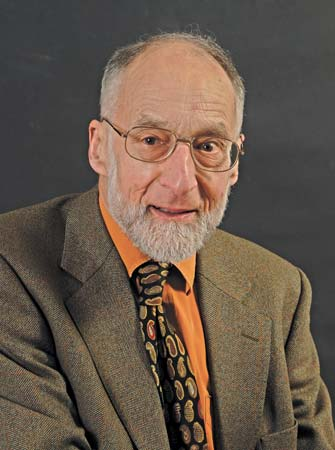
\includegraphics[width=0.8\textwidth]{milner.jpeg}
\end{column}
\begin{column}{.50\textwidth}
\footnotesize
ACM A.M. Turing Award (1991). For three distinct and complete achievements:
    \begin{itemize}
    \item LCF, the mechanization of Scott's Logic of Computable Functions, probably the first theoretically based yet practical tool for machine assisted proof construction.
    \item ML, the first language to include polymorphic type inference together with a type-safe exception-handling mechanism.
    \item CCS, a general theory of concurrency.
    \end{itemize}

    In addition, he formulated and strongly advanced full abstraction, the study of the relationship between operational and denotational semantics.
\end{column}
\end{columns}
\end{frame}



\begin{frame}{From Hoare logic to denotational semantics}

At Swansea University (1968), Milner developed his first automatic theorem prover:

\begin{itemize}
\setlength\itemsep{2em}
\item Based on Robinson's resolution principle (1965) and Hoare-Floyd logic (1967-9).
\item Program correctness generating verification conditions.
\item Verification conditions stated as first-order logic formulae.
\item The proof of verification conditions formulae with Robinson's resolution method took too long and limited the amount of theorems to proof.
\end{itemize}

\end{frame}

\begin{frame}{From Hoare logic to denotational semantics}

\begin{itemize}
\item Around 1970, Milner gets familiars with the works of Dana Scott and Christopher Strachey that founded the theory of denotational semantics.
\vspace{0.5cm}

\begin{quote}"I could write down the syntax of a programming language in this logic and i could write the semantics in the logic"\end{quote}
\item The automated reasoning implementation of Scott's logic became Standford LCF (logic of computable functions)
\end{itemize}
\end{frame}

\begin{frame}{Stanford logic of computable functions}
\begin{itemize}
\item An interactive user-guided system.
\item Programs could be reasoned about directly via their semantics encoded in Scott's logic.
\item Based on a goal-directed reasoning.
\end{itemize}

\begin{figure}[h]
\centering
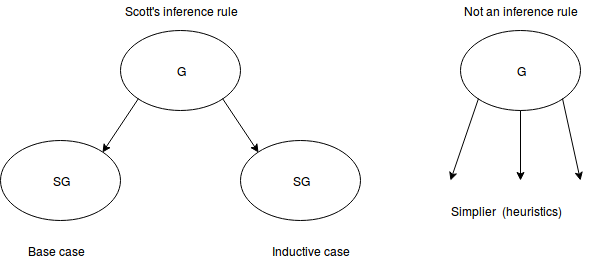
\includegraphics[width=10cm]{goal5.png}
\caption{Some commands for backwards proof in LCF}
\label{fig:error}
\end{figure} 
\end{frame}

\begin{frame}{Backward proof}
\begin{itemize}
\setlength\itemsep{2em}
\item Goal seeking activities appear in different fields. For example: Artificial Intelligence.
\item Milner worked at the time for the Stanford Artificial Intelligence Laboratory.
\item In mathematics it relates with the method of backward proof. Let's see an example:
\end{itemize}
\end{frame}

\begin{frame}
\begin{theorem}[Geometric and arithmetic means inequality]
If $x,y \in \mathbb{R^+}$ and $x \neq y$ then $\frac{x+y}{2} > \sqrt{xy}$.
\end{theorem}
\begin{proof}
\begin{align*}
\frac{x+y}{2} > \sqrt{xy} &\equiv \frac{(x+y)^2}{4} > xy \equiv && \text{x,y positive} \\
&\equiv x^2 + 2xy + y^2 > 4xy \equiv && \text{by algebra} \\
&\equiv x^2 - 2xy + y^2 \equiv && \text{by algebra} \\
&\equiv (x-y)^2 > 0 \equiv && \text{by algebra} \\
&\equiv true && \parbox[t]{5cm}{x,y are different and \\ square is positive}
\end{align*}
\end{proof}
\end{frame}

\begin{frame}{Edinburgh logic of computable functions}

The paper addresses two major issues that appeared in Standford LCF:

\begin{itemize}
\setlength\itemsep{2em}
\vspace{0.5cm}
\item The lack of any way for users to add new proof commands.
\item Large proofs could exhaust available memory.
\end{itemize}
\vspace{0.5cm}
His ideas were implemented in the Edinburgh LCF (went to Edinburgh in 1973).
\end{frame}


\section{A theory of goal seeking}

\begin{frame}{Introducing new concepts in the design of proof assistants}
The paper presents many of the core ideas underlying modern proof assistants:

\begin{itemize}
\setlength\itemsep{1em}
\item Functional programming language as a proof assistant metalanguage.
\item Representing terms, formulae and theorems of a logic as metalanguage data types.
\item Programming language types to ensure soundness. 
\item Tactics as metalanguage functions for representing subgoaling strategies.
\item Higher-order functions for combining tactics.
\end{itemize}
\end{frame}

\begin{frame}{Milner's theory of tactics}
The theory of tactics relies on the following definitions:

Let's denote the type of formulas by F, the type of goals by G, the type of procedures by P and the type of events by E.

\begin{table}[H]
\small
\begin{tabular}{|| c | c | c | c ||}
\hline
\hline Name & Type &  Notation & Meaning \\
\hline goal & List[F] $\times$ F & ($\Gamma$,F) & $\Gamma \vdash F$ unproved \\
\hline event & List[F] $\times$ F & ($\Delta$,G) & $\Delta \vdash G$ proved \\
\hline tactic & \scriptsize{G $\rightarrow$ List[G] $\times$ P} & \scriptsize{T(G) = ([$G_1;\cdots;G_n$],P)} & \\
\hline procedure & List[E] $\rightarrow$ E & P([$E_1;\cdots;E_n$]) & \\
\hline achieve & E $\times$ G & \scriptsize{achieves(($\Delta$,G),($\Gamma$,F))} & \scriptsize{$\exists \Gamma' \subseteq \Gamma$:($\Delta$,G) = ($\Gamma'$,F)} \\
\hline
\end{tabular}
\vspace{0.5cm}

\begin{itemize}
\item Equality for achieves relation is up to rename of bound variables.
\item Functions here are considered to be partial functions.
\end{itemize}
\end{table} 

\end{frame}

\begin{frame}{Milner's theory of tactics}
\begin{definition}[Validity of tactics]
A tactic $T$ is valid if whenever $T(G) = ([G_1;\cdots;G_n],P)$ and if $E_i$ achieves $G_i$ then $P([E_1;\cdots;E_n])$ is defined and achieves $G$. \\
\end{definition}

\begin{definition}[Solving a goal]
If a valid tactic $T$ verifies $T(G) = ([],P)$ then $T$ is said to solve the goal $G$ and $P([])$ should evaluate to an event that achieves $G$.
\end{definition}
\end{frame}


\begin{frame}{Using types to ensure logical soundness}

What is the relation between a goal and events?
\vspace{0.5cm}
\begin{itemize}
\setlength\itemsep{2em}
\item The two have a type $List[F] \times F$
\item However, an event has an abstract type (meaning it cannot be instantiated directly).
\item ML type-checker ensures that only functions representing sound inference rules in Scott's logic can create new events. 
\end{itemize}
\end{frame}


\begin{frame}{Saving space by not storing proofs}
\begin{itemize}
\setlength\itemsep{2em}
\item Standford LCF created a proof tree stored in computer's memory. 
\item Each proof command expands this tree by adding generated subgoals.
\item The validation procedure solves exhaustion of memory problems.
\end{itemize}
\end{frame}

\begin{frame}{Milner's theory of tactics}
\begin{figure}[h]
\centering
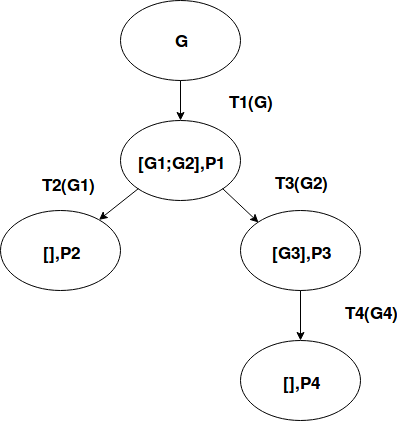
\includegraphics[width=6cm]{goal6.png}
\caption{Tactics applications}
\label{fig:error}
\end{figure}
\end{frame}

\begin{frame}{Milner's theory of tactics}
\begin{figure}[h]
\centering
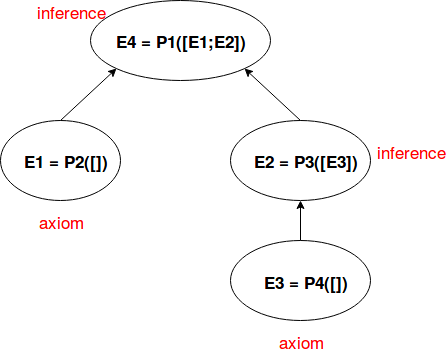
\includegraphics[width=6cm]{goal7.png}
\caption{Validations applications}
\label{fig:error}
\end{figure}
\end{frame}

\begin{frame}{Examples of tactics}
\begin{table}[H]
\begin{tabular}{|| c | c | c | c | c||}
\hline
\hline Name & Goal &  Subgoal & Validation \\
\hline GENTAC & ($\Gamma$,$\forall x. F$) & ($\Gamma$,F) & $x \notin free(\Gamma)$ \\
\hline DISCHTAC & ($\Gamma$,$A \implies B$) & ($\Gamma \cup A$,$B$) & implication rule \\
%\hline RESTAC
%\hline SIMPTAC
\hline
\end{tabular}
\caption{Primitive tactics}
\end{table}
\end{frame}

\begin{frame}{Tacticals}
\begin{itemize}
\setlength\itemsep{2em}
\item Allow to introduce new proof commands in LCF (solves first issue).
\item Requires higher-order functions in metalanguage ML.
\item Combination of tactics require exception-handling mechanism for inapplicable tactics. 
\item Example: induction tactic applied to goal that cannot be decomposed into basis and step subgoals. 
\end{itemize}
\end{frame}


\begin{frame}{Example of tacticals}

Let's denote by T the type of tactics.
\begin{table}[H]
\small
\begin{tabular}{|| c | c | c | c||}
\hline
\hline Name & Argument type & Meaning & Validation \\
\hline THEN & $T \times T$ & flatten$(T_2(T_1(G)))$ & $P_1 \circ P_2$ \\
\hline THENL & $T \times List[T]$ & flatten($List[T]$ map $T_1(G)$) & $P_1 \circ P_i$ \\
\hline ORELSE & $T \times T$ & $(T_1.getOrElse(T_2))(G)$ & succeed(P) \\
\hline REPEAT & $T$ & map T until failure or $\emptyset$ & $P^{\text{successes}}$\\
\hline
\end{tabular}
\caption{Simple tacticals}
\end{table}
\end{frame}

\begin{frame}{Composition of tacticals}
\begin{itemize}
\setlength\itemsep{2em}
\item A tactic that repeatedly strips off leading universal quantifiers and assumes the antecedent of any implication in the goal formula.
\item A goal $(\Gamma,\forall x. F_1 \implies \forall y,z. F_2 \implies F_3)$ 
\item Transformed into $(\Gamma \cup \{ F_1,F_2 \},F_3)$.
\item REPEAT ( GENTAC ORELSE DISCHTAC )
\end{itemize}
\end{frame}

\begin{frame}{Complex tactics and tacticals}
\begin{itemize}
\item Some complex tactics and tacticals that were not presented before:

	\begin{itemize}
	\item Full automatic proof methods can be implemented as tactics. 
	\item Example: RESTAC (Robinson resolution method)
	\item SIMPTAC: a simplification tactic based upon a collection of equational theorems of the form 		$\Gamma \vdash t_1 = t_2$.
	\item Tactics implementing induction and case analysis.
	\end{itemize}

\item Specialized tactics leading to a "tower" of theories (discussed later).
\item Special importance may have polymorphic theories. Example: trees with parametrized nodes.
\end{itemize}
\end{frame}

\begin{frame}{Using types to ensure logical soundness}
\begin{itemize}
\setlength\itemsep{2em}
\item The validation procedures produced by tactics actually create new theorems.
\item How are we sure that the produced theorems are correct?
\item The key again is that the type system does not allow to generate a false event. 
\end{itemize}
\end{frame}



\section[]{An example: a theorem about parsing}

\begin{frame}{Notation}
\begin{itemize}
\setlength\itemsep{2em}
\item We introduce a slightly more complex notation for sequents ($\Gamma$,F) as ($\Gamma$,F,S)
\item S is a set of equational assumptions for simplification by SIMPTAC
\item Other rules may add suitable equations to S
\item Example: if DISCHTAC has an equational antecedent then it is added to $\Gamma$ and S.
\end{itemize}
\end{frame}

\begin{frame}{The tower of theories}
\begin{figure}[h]
\centering
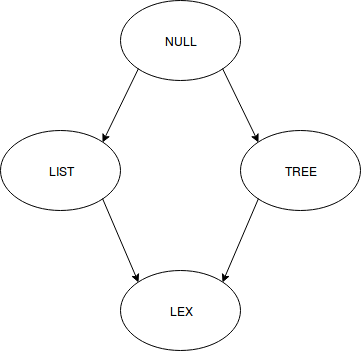
\includegraphics[width=6cm]{tower3.png}
\caption{The tower of theories in our example}
\label{fig:error}
\end{figure}
\end{frame}

\begin{frame}{The null theory}
We create the different theories as daughters of the NULL or pure theory. This theory:
\vspace{0.5cm}

\begin{itemize}
\setlength\itemsep{2em}
\item Does not contain non-logical types, constants or axioms.
\item Possesses a type ONE.
\item The only proper member object is denoted by the constant "nothing" symbol ().
\end{itemize}
\end{frame}

\begin{frame}{Polymorphic theory of lists}
\begin{itemize}
\setlength\itemsep{2em}
\item Define a unary type constructor, LIST.
\item Introduce two constants with polymorphic types:
	\begin{itemize}
	\item NIL: $\alpha$ LIST
	\item CONS: $\alpha \rightarrow \alpha$ LIST $\rightarrow \alpha$ LIST
	\end{itemize}
\item Define function APPEND: $\alpha$ LIST $\rightarrow \alpha$ LIST $\rightarrow \alpha$ LIST.
\item We characterize the LIST constructor by the isomorphism:

	$\alpha$ LIST $\simeq$ ONE + $\alpha \times \alpha$ LIST.
	
\item We characterize the constants writing equations such as: 

	APPEND( CONS a x ) y = CONS a ( APPEND x y )	
\end{itemize}
\end{frame}

\begin{frame}{Polymorphic theory of trees}
\begin{itemize}
\setlength\itemsep{2em}
\item Define a binary type constructor, TREE.
\item We characterize the TREE constructor by the isomorphism:

	\scriptsize{($\alpha,\beta$) TREE $\simeq$ $\alpha$ + $\beta \times$ ($\alpha,\beta$) TREE + $\beta \times$ ($\alpha,\beta$) TREE $\times$ ($\alpha,\beta$) TREE}.
\normalsize
\item Introduce three constants for the three tree constructors:
	\begin{itemize}
	\item TIP: $\alpha \rightarrow$ ($\alpha,\beta$) TREE
	\item NODE1: $\beta \rightarrow$ ($\alpha,\beta$) TREE $\rightarrow$ ($\alpha,\beta$) TREE
	\item NODE2: $\beta \rightarrow$ ($\alpha,\beta$) TREE $\rightarrow$ ($\alpha,\beta$) TREE $\rightarrow$ ($\alpha,\beta$) TREE
	\end{itemize}
\item Computation induction rule of Scott's logic provide us automatically with an induction rule for lists and trees. We will use a TREEINDUCTTAC in this example.
\end{itemize}
\end{frame}

\begin{frame}{Lexical theory}
\begin{itemize}
\setlength\itemsep{2em}
\item Define types ID and OP for variables and operators in the list to be parsed.
\item Define a type isomorphism that takes account of symbols ( and ) and the occurrence of an operator as a unary or binary function:

	SYMB $\simeq$ ONE + ONE + ID + OP + OP
\item We introduce and axiomatize five constructors:
	\begin{itemize}
	\item LB :SYMB
	\item RB :SYMB 
	\item VAR :ID	$\rightarrow$ SYMB
	\item UNARY :OP $\rightarrow$ SYMB
	\item BINARY :OP $\rightarrow$ SYMB
	\end{itemize}
\end{itemize}	
\end{frame}

\begin{frame}{Parsing algorithm}
\begin{itemize}
\setlength\itemsep{2em}
\item We express the parsing algorithm as a set of axioms about a function PARSE.
\item The type of PARSE is PARSE: SYMB LIST $\rightarrow$ (ID,OP) TREE $\times$ SYMB LIST.
\item The symbol list begins with a well formed formula.
\item The resulting pair is made with the shortest initial segment of the argument that is parsable, together with the remainder of the argument string.
\item A parse tree will be a tree with tips labelled in ID and whose nodes are labelled in OP.
\end{itemize}
\end{frame}


\begin{frame}{Parsing algorithm}
\begin{itemize}
\setlength\itemsep{2em}
\item We express the parsing algorithm as a set of axioms about a function PARSE.
\item The type of PARSE is PARSE: SYMB LIST $\rightarrow$ (ID,OP) TREE $\times$ SYMB LIST.
\item The symbol list begins with a well formed formula.
\item The resulting pair is made with the shortest initial segment of the argument that is parsable, together with the remainder of the argument string.
\item A parse tree will be a tree with tips labelled in ID and whose nodes are labelled in OP.
\end{itemize}
\end{frame}

\begin{frame}{Parse example}
\begin{figure}[h]
\centering
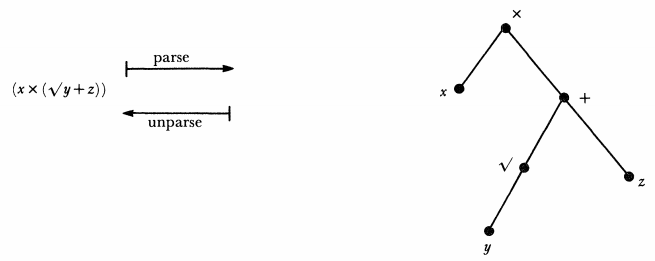
\includegraphics[width=10cm]{tree.png}
\caption{An example of parse and unparse}
\label{fig:error}
\end{figure}
\end{frame}

\begin{frame}{Axioms for PARSE}
Take $x \in ID$, $f \in OP$, $s \in SYMB LIST$ and $t \in (ID,OP) TREE$. Then:
\begin{itemize}
\setlength\itemsep{2em}
\item PARSE ( CONS ( VAR x ) s ) = ( TIP x, s )
\item PARSE ( CONS ( UNARY f ) s ) = ( NODE1 f t',s' ) 
		WHERE (t',s') = PARSE s

\item PARSE ( CONS LB s ) = PARSETWO t' s' \\
		WHERE (t',s') = PARSE s
		
\item PARSETWO t ( CONS ( BINARY f ) s ) = \\ \hspace{0.5em} ( NODE2 f t t', CHECKRB s' ) \\
		WHERE (t',s') = PARSE s 
		
\item CHECKRB ( CONS RB s) = s
\end{itemize}


For an example, parse $(a f b)$ or $(f a)$.
\end{frame}

\begin{frame}{Axioms for UNPARSE}
\begin{itemize}
\setlength\itemsep{2em}
\item The type of UNPARSE is UNPARSE:(ID,OP) TREE $\rightarrow$ SYMB LIST.
\item UNPARSE ( TIP x ) = CONS ( VAR x ) NIL
\item UNPARSE ( NODE1 f t ) = \\ \hspace{0.5em} CONS ( UNARY f ) ( UNPARSE t ) 
\item UNPARSE ( NODE2 f t t' ) = \\
		\hspace{0.5em} APPEND ( CONS LB ( UNPARSE t ) ) \\
			   \hspace{1em} ( APPEND ( CONS ( BINARY f ) ( UNPARSE t' ) ) \\
			   			\hspace{1.5em} ( CONS RB NIL)))	
\end{itemize}
\end{frame}

\begin{frame}{The theorem}
We want to proof the following theorem over a parsing problem:
\vspace{1cm}

F:$\forall t,s. $ WD[t] $\implies$ PARSE ( APPEND ( UNPARSE t ) s ) = (t,s)

\vspace{1cm}

Where WD[t] expresses that the tree t is appropriately well defined. 
\end{frame}

\begin{frame}{The tactic employed}
The intuition needed from the user is that is natural to attack this problem by:
\vspace{0.5cm}

\begin{itemize}
\setlength\itemsep{2em}
\item Structural induction upon trees.
\item Mixture of simplification by SIMPTAC and routine logical manipulation by RESTAC.
\item As implication and quantification are used: GENTAC and DISCHTAC.
\item It is reasonable to expect that WD[t] has been proved in advanced in OTHER THEORIES.
\end{itemize}
\end{frame}

\begin{frame}
Let's represent by L the set of auxiliary lemmas coming from WD[t]. 
\vspace{1cm}

The tactic goes as follows: 

\vspace{1cm}
\scriptsize


USELEMMASTAC (L) THEN \\
TREEINDUCTAC THEN SIMPTAC THEN \\
REPEAT (GENTAC ORELSE DISCHTAC) THEN \\
RESTAC THEN SIMPTAC \\


\end{frame}

\begin{frame}
It is claimed that: \vspace{1cm} 

\begin{quote} The combination of tactics used was remarkably similar to that which succeeded on other problems, in totally different problem domains. \textbf{The difference was mainly in the particular induction rule used, in the particular auxiliary lemmas employed and in the particular simplification rules embodied in the main goal G.} \end{quote}
\end{frame}

\section{Posterior developments}

\begin{frame}{Influences in other proof assistants}
LCF influenced the creation of posterior proof assistants such as:

\begin{itemize}
\setlength\itemsep{2em}
\item Cambridge LCF (Paulson, 1987): enriched LCF logic and rewriting and tactics techniques.
\item Nuprl, Constructions and Petersson's Programming system for Type Theory
	\begin{itemize}
	\setlength\itemsep{2em}
	\item Based on the LISP implementation of ML in Edinburgh LCF.
	\item Tactics were modified to validate goals with representations of proofs rather than theorems.
	\end{itemize}
\end{itemize}
\end{frame}

\begin{frame}{Influences in other proof assistants}
LCF influenced the creation of posterior proof assistants such as:

\begin{itemize}
\setlength\itemsep{2em}
\item HOL (Gordon, 1993):  and 
	\begin{itemize}
	\setlength\itemsep{2em}
	\item Based on the LISP code implementing Cambridge LCF.
	\item Tactics were adapted for classical higher-order logic rather than for Scott's logic.
	\end{itemize}
\item Isabelle (Paulson, 1990):
	\begin{itemize}
	\setlength\itemsep{2em}
	\item A generic tool to create proof assistants by instantiating a logical framework.
	\item No need to create a system for each modification of LCF.
	\item Tactics and tacticals operate on proof states rather than on subgoals.
	\end{itemize}
\end{itemize}
\end{frame}

\begin{frame}{How tactics survived LCF}
On the one hand...

\begin{itemize}
\setlength\itemsep{2em}
\item  Scott's logic was less suitable for verifying hardware or checking general mathematical proofs.
\item It was tactics and typed programmable metalanguage for ensuring logical soundness rather than LCF logic that had a major impact on modern theorem proving.
\item Descendants of LCF underlie the majority of proof assistants today.
\end{itemize}

\end{frame}

\begin{frame}
on the other hand...

\begin{itemize}
\setlength\itemsep{2em}
\item Programming algorithms as derived rules or tactics is more complicated than programming them directly. 
\item  Resulting implementations had poor performance. 
\item PVS or ACL2 showed better performance than LCF systems. 
\item Does LCF's performance penalty worth logical soundness? 
\end{itemize}
\end{frame}

\begin{frame}{Progress in machine checked proofs}
Some machine proofs made with tactic-based proof assistants:

\begin{itemize}
\setlength\itemsep{2em}
\item HOL: ARM6 processor (2003)
\item Coq: four colour theorem (2007), cryptographic proofs (Barthe et alii., 2009), CompCertC compiler (2009), Feit-Thomson theorem (2013)
\item Isabelle: correctness of security protocols (Paulson, 1998), seL4 operating system(2009), Gödel's second incompleteness theorem (2014)
\item HOL/Isabelle: Kepler conjecture on sphere packing (2014)
\end{itemize}
\end{frame}

\begin{frame}{The tower of theories}
In the paper, Milner establishes the need to keep a "tower of theories" that would...

\begin{itemize}
\setlength\itemsep{2em}
\item Allow us to define different knowledge in each problem or theory where we are working.
\item Allow us access to those theorems previously defined.
\item The use of this "tower" should decrease the time needed to prove new results.
\end{itemize}
\end{frame}

\begin{frame}
\begin{figure}[h]
\centering
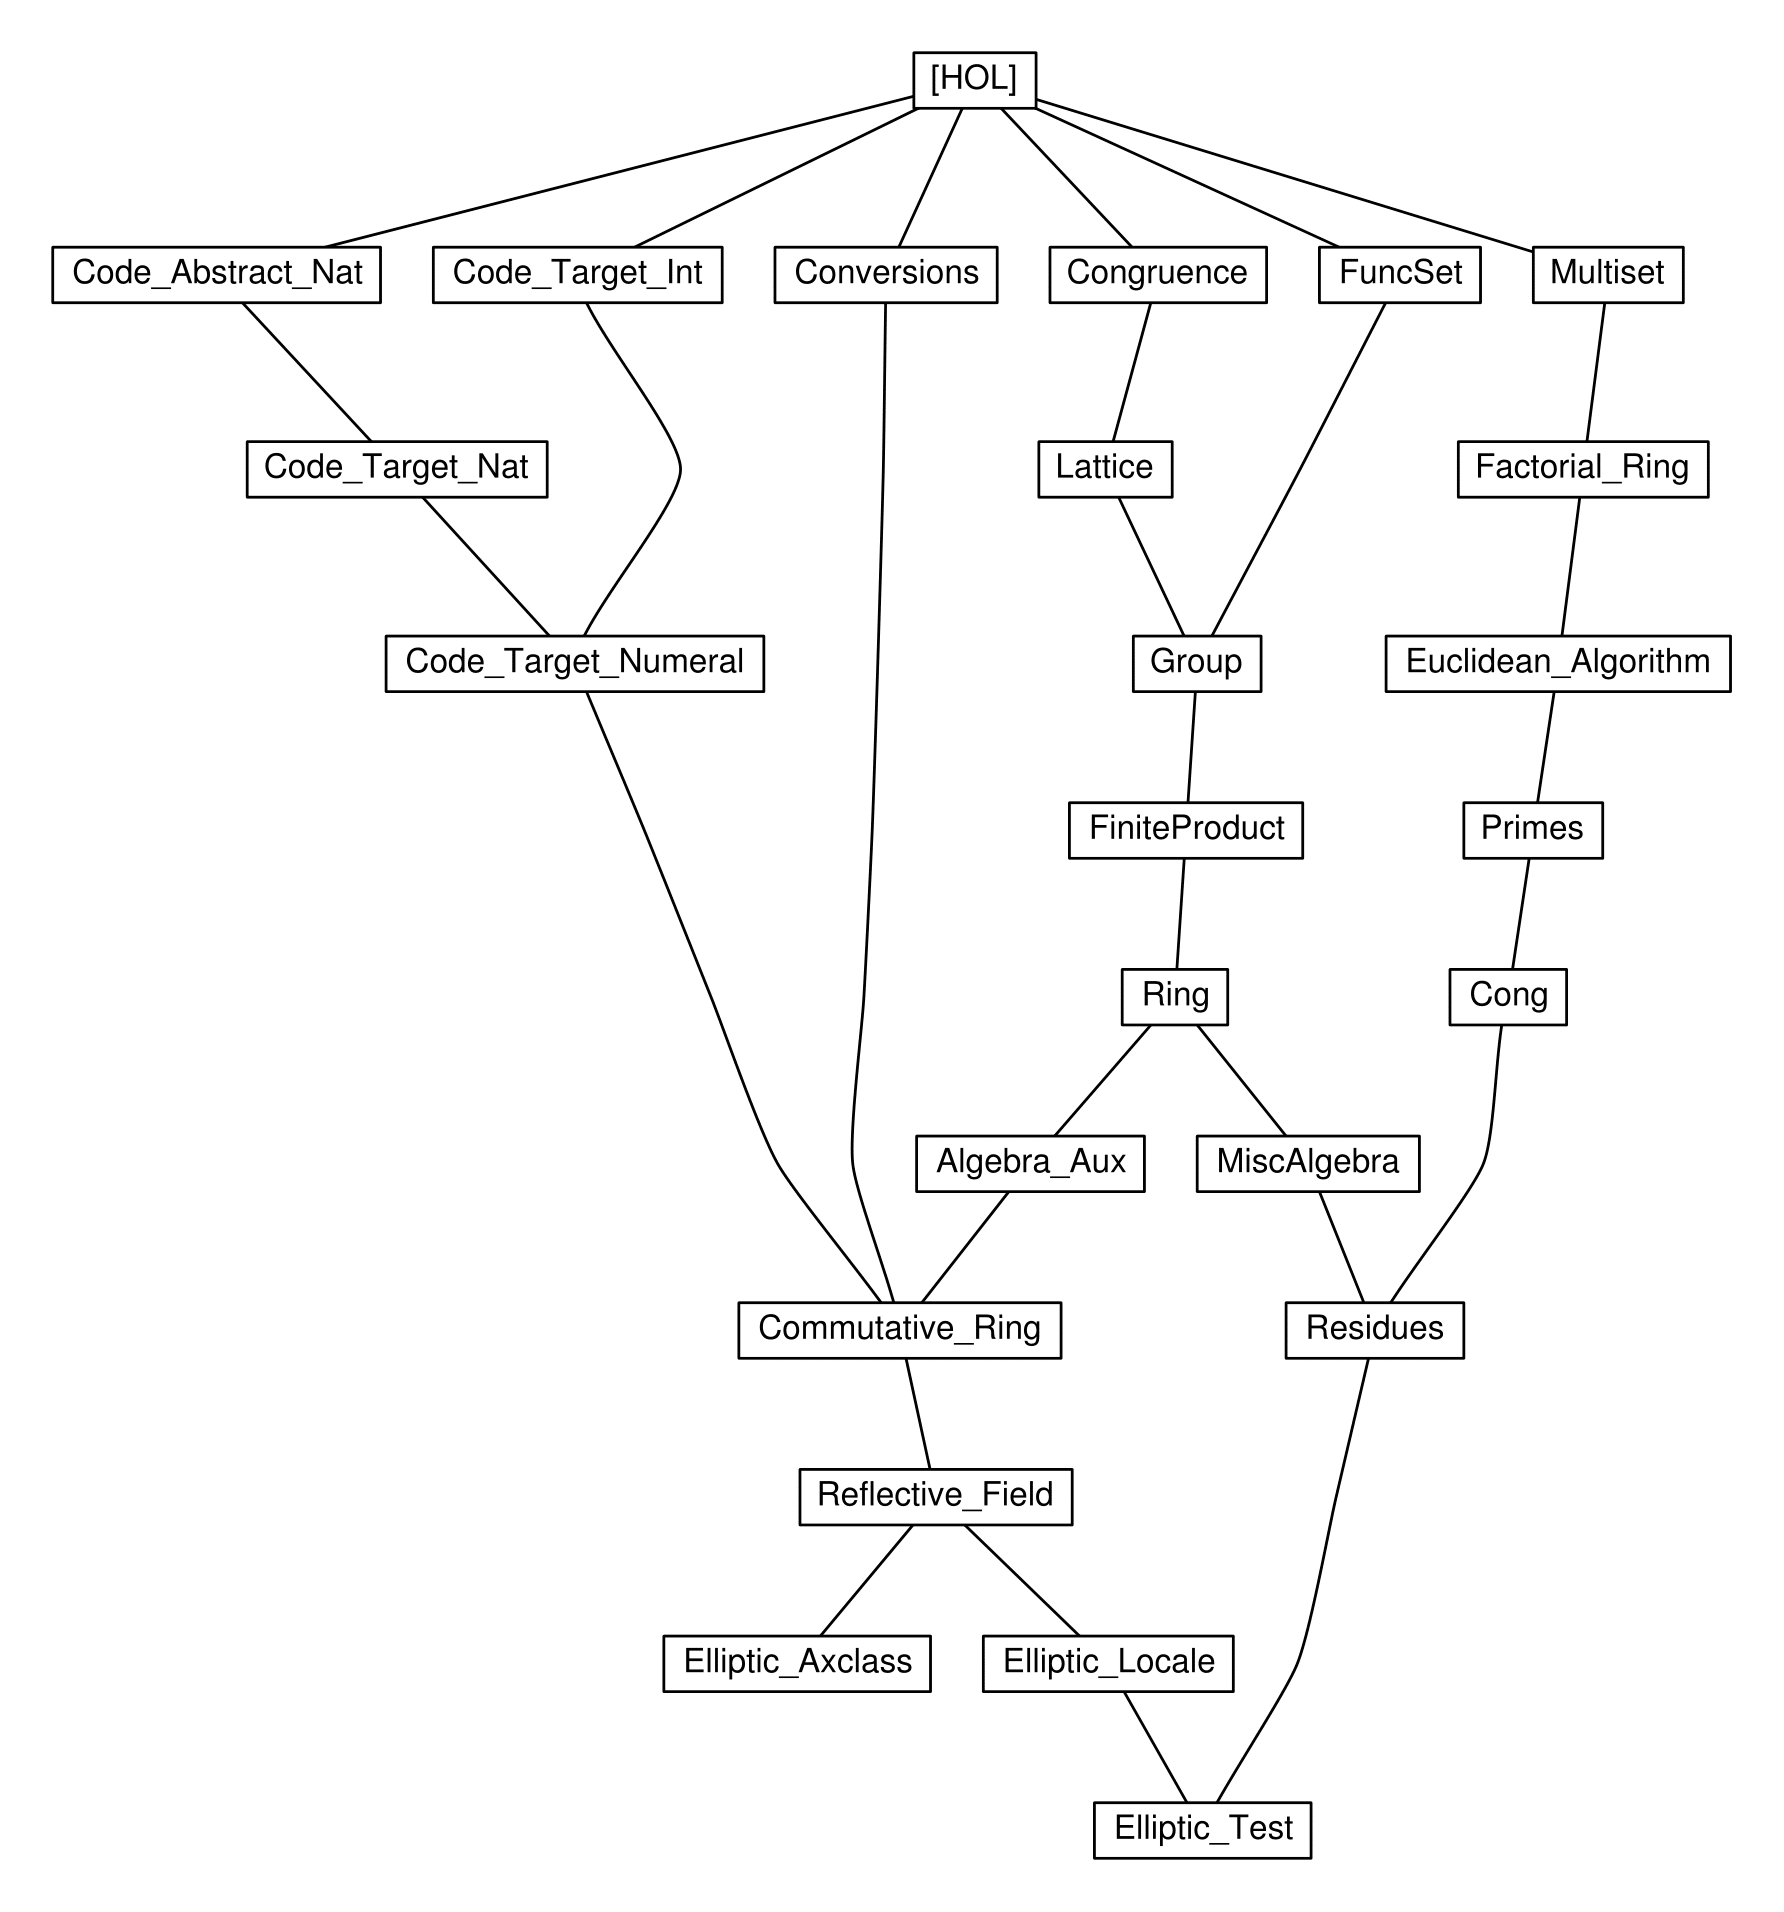
\includegraphics[width=7cm]{tower.png}
\caption{Theory tower for a proof about elliptic curves in Isabelle}
\label{fig:error}
\end{figure}
\end{frame}

\begin{frame}{Inconveniences of the tower of theories}
The model of the tower of theories has of course limitations:

\begin{itemize}
\setlength\itemsep{2em}
\item Every new proof assistant should start its theories from scratch...
\item unless we accept the use of different proof assistants for proofs. 
\item The proof that two different proof assistants can be combined to obtain certain results is not necessarily trivial.
\end{itemize}
\end{frame}

\begin{frame}{Influence in programming languages}
The characteristics that we have explored on ML made it suitable as a base for other functional languages such as:

\begin{itemize}
\setlength\itemsep{2em}
\item Standard ML (metalanguage in Isabelle and several HOL systems)
\item OCaml (metalanguage for Coq and HOL Light)
\item F\# initially derived from OCaml
\end{itemize}
\end{frame}

\section{Conclusion and references}

\begin{frame}{Conclusion}
\begin{quote}"It emerges from these various studies that the method of composing proof tactics, which is illustrated in this paper on a rather simple example, not only provides a means of communicating proof methods to a machine, and of tuning them to particular needs, but also presents to mathematicians and engineers \textbf{a lucid way of communicating such methods among themselves}."\end{quote}

\scriptsize \centerline{Intuition $\rightarrow$ Formalization?}
\end{frame}

\begin{frame}{References}
\nocite{*}
\printbibliography
\end{frame}

\begin{frame}{}
\begin{center}
\Huge Questions?
\end{center}
\end{frame}




\end{document}